%% Diambil dari buku Data and Computer Communications, 8th Edition
\chapter{Data Link Control Protocol}


\section{Key Points}

\begin{itemize}
	\item Karena kemungkinan kesalahan transmisi, dan karena penerima data (\textit{receiver}) mungkin perlu mengatur kecepatan kedatangan data (\textit{data rate}), maka tidak cukup hanya dengan teknik sinkronisasi dan antarmuka (\textit{interface}). Perlu untuk menerapkan lapisan kontrol (\textit{layer of control}) di setiap perangkat komunikasi yang menyediakan fungsi seperti kontrol aliran (\textit{flow control}), deteksi kesalahan (\textit{error detection}), dan kontrol kesalahan (\textit{error control}). Lapisan kontrol (\textit{layer of control}) ini dikenal sebagai \textit{data link control protocol}.

	\item \textit{Flow control} memungkinkan penerima (\textit{receiver}) untuk mengatur aliran data dari pengirim sehingga \textit{buffer} penerima tidak meluap (\textit{overflow}).
	
	\item Dalam \textit{data link control protocol}, \textit{error control} dicapai dengan transmisi ulang \textit{frame} rusak yang belum diakui atau yang meminta transmisi ulang oleh pihak lain.
	
	\item \textit{High-level data link control} (HDLC) adalah \textit{data link control protocol} yang banyak digunakan. Ini berisi hampir semua fitur yang ditemukan di \textit{data link control protocol} lainnya.
\end{itemize}


\section{Pengantar}

Diskusi kita sejauh ini berkaitan dengan pengiriman sinyal melalui tautan transmisi (\textit{transission link}). Untuk komunikasi data digital yang efektif, lebih banyak yang dibutuhkan untuk mengontrol dan mengelola pertukaran data. Dalam bab ini, kami mengalihkan penekanan kami ke pengiriman data melalui tautan komunikasi data (\textit{data communication link}). Untuk mencapai kontrol yang diperlukan, lapisan logika (\textit{layer of logic}) ditambahkan di atas \textit{physical layer} yang dibahas dalam Bab \ref{ch:06}; logika ini disebut sebagai \textit{data link control} atau \textit{data link control protocol}. Ketika \textit{data link control protocol} digunakan, media transmisi antar sistem disebut sebagai \textit{data link}.

Untuk melihat kebutuhan terhadapt \textit{data link control}, kami membuat daftar beberapa persyaratan dan tujuan untuk komunikasi data yang efektif antara dua stasiun pemancar dan penerima yang terhubung langsung:

\begin{itemize}
	
	\item \textit{Frame synchronization}: Data dikirim dalam blok yang disebut \textit{frame}. Bagian awal dan akhir setiap \textit{frame} harus dapat dikenali. Kami secara singkat memperkenalkan topik ini dengan diskusi tentang \textit{synchronous frames} (Gambar \ref{fig:06.02}).

	\item \textit{Flow control}: Stasiun pengirim tidak boleh mengirim \textit{frame} dengan kecepatan yang lebih cepat daripada yang dapat diserap oleh stasiun penerima.
	
	\item \textit{Error control}: \textit{Bit error} yang diperkenalkan oleh sistem transmisi harus diperbaiki.
	
	\item \textit{Addressing}: Pada sebuah \textit{shared link}, seperti \textit{local area network} (LAN), identitas dari dua stasiun yang terlibat dalam transmisi harus ditentukan.
	
	\item \textit{Control} dan data pada \textit{link} yang sama: Biasanya tidak diinginkan untuk memiliki jalur komunikasi yang terpisah secara fisik untuk \textit{control information}. Oleh karena itu, penerima harus dapat membedakan \textit{control information} dari data yang dikirim.
	
	\item \textit{Link management}: Inisiasi, pemeliharaan, dan penghentian pertukaran data yang berkelanjutan membutuhkan koordinasi dan kerja sama yang cukup di antara stasiun. Prosedur untuk pengelolaan pertukaran ini diperlukan.
\end{itemize}

Tak satu pun dari persyaratan ini dipenuhi oleh teknik yang dijelaskan dalam Bab \ref{ch:06}. Kita akan melihat dalam bab ini bahwa \textit{data link protocol} yang memenuhi persyaratan ini adalah hal yang agak rumit. Kami mulai dengan melihat dua mekanisme utama yang merupakan bagian dari \textit{data link control}: \textit{flow control} dan \textit{error control}. Mengikuti latar belakang ini, kami melihat contoh terpenting dari \textit{data link control protocol}: HDLC (\textit{high-level data link control}). Protokol ini penting karena dua alasan: Pertama, ini adalah standar \textit{data link control protocol} yang banyak digunakan. Kedua, HDLC berfungsi sebagai \textit{baseline} yang mana hampir semua \textit{data link control protocol} penting lainnya diturunkan. Akhirnya, lampiran bab ini membahas beberapa masalah kinerja yang berkaitan dengan \textit{data link control}.


\section{Flow Control}

\textit{Flow control} adalah teknik untuk memastikan bahwa entitas pengirim tidak membanjiri entitas penerima dengan data. Entitas penerima biasanya mengalokasikan \textit{buffer data} dengan beberapa panjang maksimum untuk transfer. Saat data diterima, penerima harus melakukan sejumlah pemrosesan sebelum meneruskan data ke \textit{software} tingkat yang lebih tinggi. Jika tidak ada \textit{flow control}, \textit{buffer} penerima mungkin terisi dan meluap saat memproses data lama.

Untuk memulai, kami memeriksa mekanisme \textit{flow control} jika tidak ada \textit{error}. Model yang akan kita gunakan digambarkan pada Gambar \ref{fig:07.01}a, yang merupakan diagram urutan waktu vertikal. Ini memiliki keuntungan dalam menunjukkan ketergantungan waktu dan menggambarkan hubungan kirim-terima yang benar. Setiap panah mewakili satu frame yang menghubungkan tautan data antara dua stasiun. Data dikirim dalam urutan bingkai, dengan setiap bingkai berisi sebagian data dan beberapa informasi kontrol. Waktu yang dibutuhkan stasiun untuk memancarkan semua bit frame ke medium adalah waktu transmisi; ini sebanding dengan panjang frame. Waktu propagasi adalah waktu yang dibutuhkan sedikit untuk melintasi tautan antara sumber dan tujuan. Untuk bagian ini, kami berasumsi bahwa semua frame yang dikirimkan berhasil diterima; tidak ada bingkai yang hilang dan tidak ada yang datang dengan kesalahan. Selain itu, bingkai tiba dalam urutan yang sama seperti saat dikirim. Namun, setiap frame yang ditransmisikan mengalami jumlah penundaan yang berubah-ubah dan variabel sebelum penerimaan.\footnotemark

\footnotetext{ 
	Pada direct point-to-point link, jumlah \textit{delay} telah ditetapkan sebelumnya, bukan suatu variabel. Namun, \textit{data link control protocol} dapat digunakan melalui koneksi jaringan, seperti \textit{circuit-switched} atau jaringan ATM, dalam hal ini penundaan dapat bervariasi.
}

\begin{figure}
	\centering
	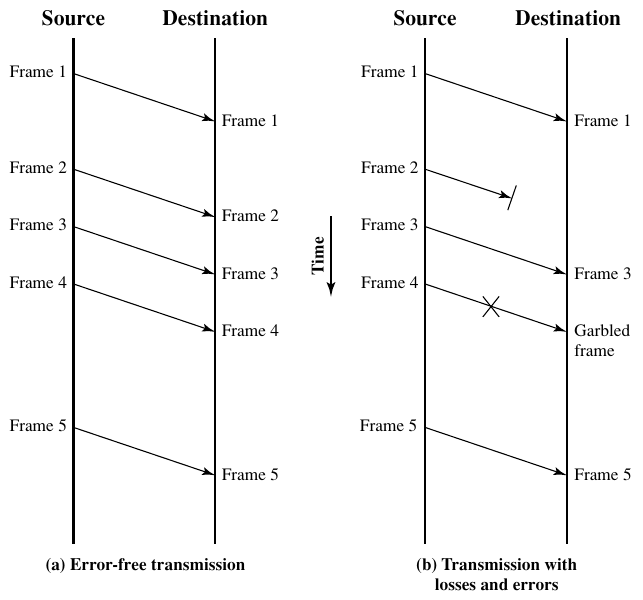
\includegraphics[width=0.8\linewidth]{gambar/fig:07.01}
	\caption{Model dari Frame Transmission}
	\label{fig:07.01}
\end{figure}

\subsection{Stop-and-Wait Flow Control}

\textit{Flow control} yang paling sederhana adalah \textbf{stop-and-wait flow control}. Cara kerja dari \textit{flow control} ini adalah sebagai berikut. Sebuah sumber akan mentransmisikan sebuah \textit{frame}. Setelah sebuah penerima memperoleh \textit{frame} tersebut, penerima ini akan menunjukkan kesediaan untuk menerima \textit{frame} yang lain dengan cara mengirimkan kembali \textit{acknowledgment} ke \textit{frame} yang baru saja diterima. Sumber tersebut harus menunggu hingga \textit{acknowledgment} ia terima sebelum mengirimkan \textit{frame} selanjutnya. Penerima dapat menghentikan aliran data dengan cara menahan \textit{acknowledgment}. Prosedur ini bekerja dengan baik dan berat untuk ditingkatkan ketika pesan yang dikirim dalam ukuran \textit{frame} yang besar. Namun untuk beberapa kasus, sumber akan memecah blok data yang besar menjadi blok data yang lebih kecil dan mentransmisikan data dalam \textit{frame} yang banyak. Hal ini dilakukan karena alasan sebagai berikut:

\begin{itemize}
	\item Ukuran \textit{buffer} dari \textit{receiver} itu terbatas.
	\item Semakin lama transmisinya, semakin besar kemungkinan terjadinya \textit{error}, yang mengharuskan keseluruhan frame untuk ditransmisikan kembali. Dengan \textit{frame} yang lebih kecil, \textit{error} dapat dideteksi lebih awal, dan jumlah data yang lebih kecil yang perlu ditransmisikan kembali.
	\item Pada \textit{shared medium}, seperti LAN, biasanya diinginkan untuk tidak mengizinkan satu \textit{station} menempati media dalam waktu yang lama, sehingga menyebabkan penundaan yang lama di \textit{station} pengirim lainnya.
\end{itemize}

Dengan menggunakan \textit{multiple frame} untuk satu pesan, prosedur \textit{stop-and-wait} mungkin tidak cukup. Karena permasalahannya adalah hanya satu frame yang dapat ditransmisikan pada satu waktu. Lebih jelasnya, pertama-tama kita tentukan panjang bit dari link-nya:

\begin{equation}\label{pers.07.01}
	B = R \times \frac{d}{V}
\end{equation}\\
dimana

\begin{itemize}
	\item[$ B = $] Panjang dari \textit{link} dalam bit; ini adalah jumlah bit yang ada di link pada saat stream dari bit sepenuhnya menempati link.
	\item[$ R = $] \textit{Data rate} dari link, dalam bps.
	\item[$ d = $] Panjang, atau jarak, dari link, dalam bps.
	\item[$ V = $] Kecepatan propagasi, dalam m/s.
\end{itemize}

Ketika panjang bit dari link lebih besar daripada panjang frame, maka dapat menghasilkan ketidakefisien yang serius. Seperti yang ditunjukkan oleh Gambar \ref{fig:07.02}, waktu transmisi (waktu yang dibutuhkan untuk station mentransmisikan sebuah frame) dinormalisasikan ke 1, dan delay propagasi (waktu yang dibutuhkan sebuah bit berjalan dari pengirim ke penerima) yang diekspresikan sebagai variabel $ a $. Sehingga,

\begin{equation}\label{pers.07.02}
	a = \frac{B}{L}
\end{equation} \\
dimana $ L $ adalah jumlah bit dalam sebuah frame (panjang dari sebuah frame dalam bit).

\begin{figure}
	\centering
	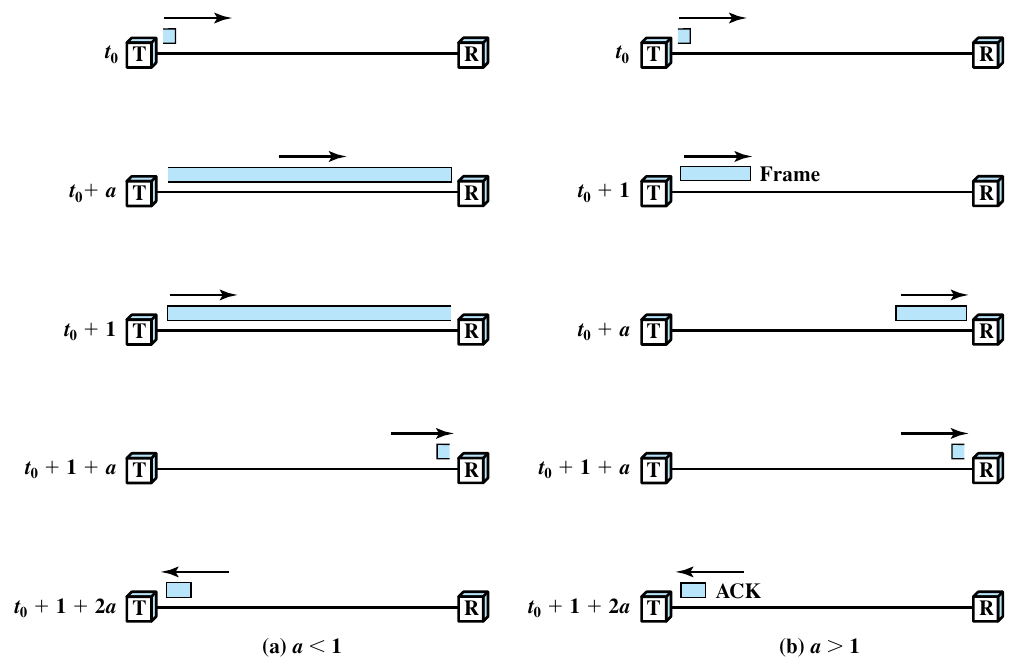
\includegraphics[width=\linewidth]{gambar/fig:07.02}
	\caption{Penggunaan Stop-and-Wait Link (waktu transmisi = 1; waktu propagasi = a)}
	\label{fig:07.02}
\end{figure}

Ketika $ a $ bernilai kurang dari 1, maka waktu propagasi lebih kecil dari waktu transmisi. Dalam hal ini, \textit{frame} cukup panjang sehingga bit pertama dari \textit{frame} tersebut tiba di tujuan sebelum sumber selesai mentransmisikan \textit{frame}. Ketika $ a $ bernilai lebih besar dari 1, waktu propagasi lebih besar dari waktu transmisi. Dalam hal ini, pengirim menyelesaikan transmisi seluruh \textit{frame} sebelum bit terdepan dari \textit{frame} tersebut tiba di penerima. Dengan kata lain, nilai $ a $ yang lebih besar konsisten dengan \textit{data rate} dan/atau jarak yang lebih jauh antar \textit{station}.

Kedua bagian dari Gambar \ref{fig:07.02} (a dan b) terdiri dari urutan (\textit{sequence}) \textit{snapshot} dari proses transmisi dari waktu ke waktu. Dalam kedua kasus, empat \textit{snapshot} pertama menunjukkan proses transmisi \textit{frame} yang berisi data, dan \textit{snapshot} terakhir menunjukkan kembalinya \textit{acknowledgment frame}. Perhatikan saat $ a > 1 $, saluran selalu kurang dimanfaatkan dan bahkan saat \textit{a < 1}, saluran digunakan secara tidak efisien. Intinya, untuk \textit{data rate} yang sangat tinggi, untuk jarak yang sangat jauh antara pengirim dan penerima, \textit{stop-and-wait flow control} menyediakan penggunaan jalur yang tidak efisien. 

\begin{exmp}\label{exp:07.01}
	Diketahui sepanjang 200 m jalur fiber optik yang beroperasi pada 1 Gbps. Kecepatan propagasi dari fiber optik adalah $ 2 \times 10^8 $ m/s. Dengan menggunakan Persamaan \ref{pers.07.01}, $ B = (10^9 \times 200) / (2 \times 10^8) = 1000 $ bits. Kita asumsikan bahwa sebuah \textit{frame} yang berukuran 8000 bits akan ditransmisikan. Dengan menggunakan Persamaan \ref{pers.07.02}, $ a = 1000/8000 = 0.125 $. Berdasarkan Gambar \ref{fig:07.02}a, asumsikan transmisi dimulai saat $ t = 0 $. Setelah 1 $ \mu $s (normalisasi waktu dari 0.125 waktu \textit{frame}), bit pertama dari \textit{frame} telah mencapai R, dan 1000 bits pertama dari \textit{frame} telah tersebar disepanjang jalur atau \textit{link}.\\
	\indent Pada saat t = 8 $\mu$s, bit terakhir dari \textit{frame} baru saja selesai ditransmisikan oleh T dan akhir 1000 bit dari \textit{frame} telah tersebar sepanjang \textit{link}. Saat t = 9 $\mu$s, bit terakhir dari \textit{frame} tiba di R. R sekarang mengirimkan kembali ACK \textit{frame}. Jika kita asumsikan bahwa waktu transmisi \textit{frame} dapat diabaikan (ACK \textit{frame} sangat kecil), dan ACK dikirim segera, ACK tiba di T pada t = 10 $\mu$s. Pada titik ini, T dapat memulai untuk mengirimkan \textit{frame} yang baru. Waktu transmisi aktual dari \textit{frame} ini adalah 8 $\mu$s, tetapi total waktu untuk mentransmisikan \textit{frame} pertama dan diterima dan ACK adalah 10 $\mu$s.\\
	\indent Sekarang anggaplah sebuah 1-MBps link antara 2 \textit{ground station} yang berkomunikasi melalui \textit{satellite relay}. Sebuah \textit{geosynchronous satellite} memiliki altitude 36.000 km. Sehingga $ B = (10^6 \times 2 \times 36.000.000)/(3 \times 10^8) = 240.000 $ bit. Untuk sebuah \textit{frame} yang panjangnya 8000 bit, $ a = (240.000 / 8000) = 30 $. Berdasarkan Gambar \ref{fig:07.02}b, kita dapat melakukan hal yang sama seperti contoh sebelumnya. Pada kasus ini, dibutuh 240 ms untuk bit pertama dari \textit{frame} untuk tiba dan tambahan 8 ms untuk keseluruhan \textit{frame} untuk tiba. ACK tiba saat $ t = 488 $ ms. Waktu transmisi aktual untuk \textit{frame} pertama adalah 8 ms. tapi waktu keseluruhan untuk mentransmisikan \textit{frame} pertama dan meneria ACK adalah 488 ms.
\end{exmp}


\subsection{Sliding-Window Flow Control}

Inti dari permasalahan yang telah dijelaskan sejauh ini adalah bahwa hanya satu \textit{frame} pada satu waktu yang dapat transit. Di dalam situasi dimana panjang bit dari link lebih besar daripada panjang \textit{frame} ($ a > 1 $)

\section{Error Control}


\section{High-Level Data Link Control (HDLC)}
